\section{Introduction}

A multiple-choice answer hides more than one decision. A model can first narrow the field to a few answers that still seem possible and only later settle on one final winner. Standard evaluation only shows the last step. It tells us what answer came out, but not when that answer first became a serious option inside the network.

This paper asks a simple question. Does the eventual answer become one of the plausible answers before the model writes the margin that finally separates it from the runner-up? Figure~\ref{fig:flagship} previews the answer. In the pooled primary analysis, by 20\% of normalized depth the eventual answer is already in the plausible answer set for \FlagshipTwentyPlausiblePct{} of evaluable cases, but only \FlagshipTwentyCommittedPct{} are already stably committed.

We answer that question in a deliberately direct way. We build a normal multiple-choice
prompt, end it with the suffix ``\texttt{Final answer:}'', and then score the exact strings the
model could write next. On the main path, that string is the full option text itself, such
as ``\texttt{photosynthesis}''. So instead of training a separate probe to guess the answer
from hidden states, we measure the scores of the answer strings that the model is actually
being asked to produce.

Our setting is intentionally narrow and easy to audit. We evaluate nine instruction-tuned
open-weight models from the Qwen 2.5 Instruct, Gemma 2 IT, and Llama Instruct families
on \PaperPromptCount{} ARC-Challenge and CommonsenseQA questions. The claim of the
paper is limited to that setting. Within it, the pattern is consistent: the eventual answer
usually enters the plausible answer set well before it becomes stably isolated from the
runner-up. All \ArcCsqaPositiveCells{} evaluable model-dataset cells are positive under the
preregistered primary rule (Figure~\ref{fig:forest}, Table~\ref{tab:primary-summary}).

The paper makes three contributions. First, it gives a simple measurement framework for
separating ``still possible'' from ``finally chosen'' by scoring the task's own answer strings
rather than an external probe target. Second, it shows a large and consistent gap between
those two stages in the pooled curves and in every evaluable ARC-Challenge and
CommonsenseQA cell. Third, it shows that the same broad lag remains visible under two
control answer formats, even though those controls change coverage and can change the
final winner.

\begin{figure*}[t]
\centering
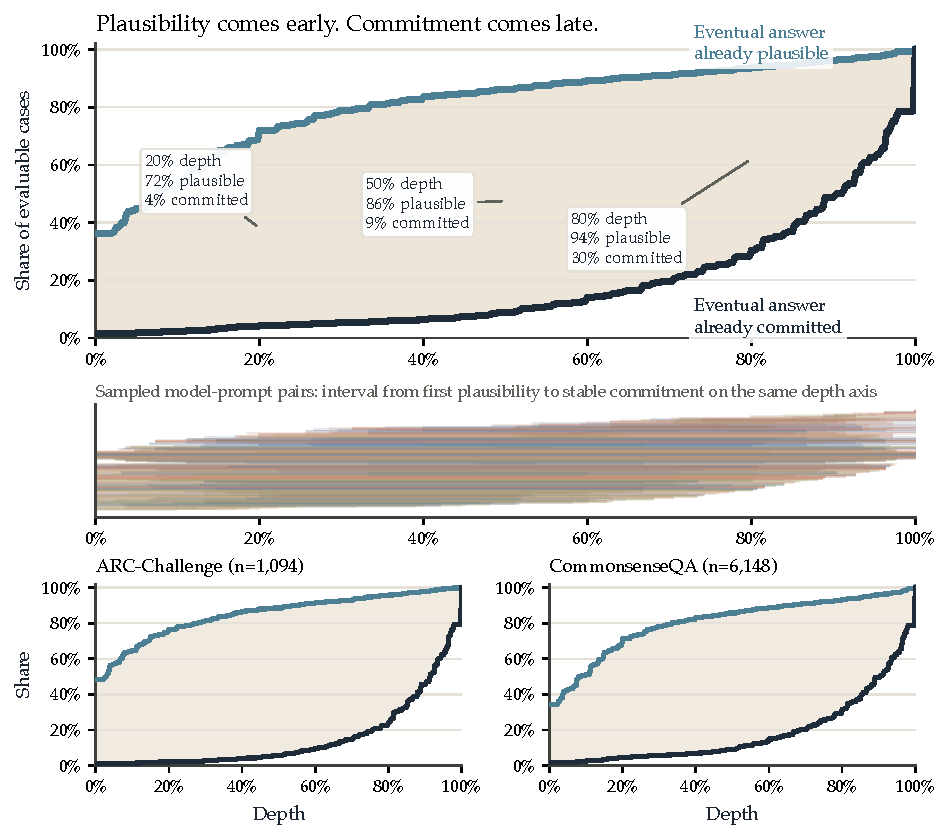
\includegraphics[width=\textwidth]{figure1_flagship_plausibility_commitment.pdf}
\caption{\textbf{The eventual answer becomes plausible much earlier than it becomes committed.} The top panel pools all evaluable model-prompt pairs from the primary analysis path (\texttt{semantic\_exact} with identity ordering). The light curve asks: by this depth, in how many cases is the eventual answer already one of the plausible answers? The dark curve asks: by this depth, in how many cases has the model already opened a stable winner-runner margin that it keeps through the end of the network? The band between the curves is the main object in the paper: cases where the answer already looks plausible but the model has not fully committed yet. The interval strip shows a sample of individual cases on the same normalized-depth axis, and the two bottom panels show the same pattern separately for ARC-Challenge and CommonsenseQA.}
\label{fig:flagship}
\end{figure*}
